\documentclass[12pt,a4paper]{report}
\usepackage[T2A]{fontenc}
\usepackage[utf8]{inputenc}
\usepackage[russian]{babel}
\usepackage[LGRgreek]{mathastext}
\usepackage{graphicx, setspace, multirow, amsmath}
\usepackage[table,xcdraw]{xcolor}
\usepackage{slashbox}

\usepackage[
top = 1.25cm,
bottom = 2.0cm]{geometry}

\makeatletter
\newcommand{\mathleft}{\@fleqntrue\@mathmargin0pt}
\newcommand{\mathcenter}{\@fleqnfalse}
\makeatother

\begin{document}
\begin{titlepage}
	\centering
    % HEADER
	{
        \scshape
        Федеральное государственное автономное образовательное учреждение высшего образования
        \par
        \textbf{«Научно-образовательная корпорация ИТМО»}
        \par
        \vspace*{1cm}
        Факультет Программной Инженерии и Компьютерной Техники
        \par
    }
    % LOGO
    \vspace*{0.6cm}
    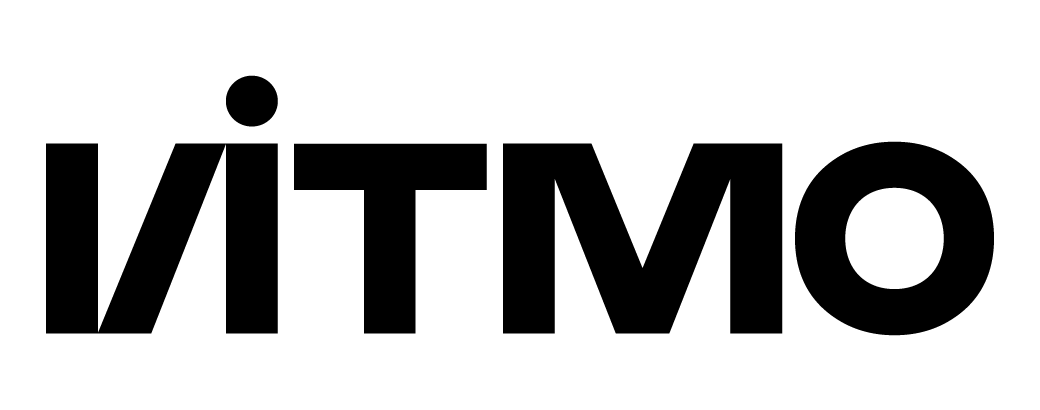
\includegraphics[width=\textwidth]{logo.png}
    % LAB INFO
    {
        \Large
        \textbf{Курсовая работа\\ <<Синтез комбинаторных схем>>\\ Часть №2}
        \par 
        \normalsize
        \vspace*{0.75cm}
        \textbf{Вариант 78}
        \par
    }
    \vfill
    % СREDITS
    \hfill\begin{minipage}{\dimexpr\textwidth-7.8cm}
        \textbf{Выполнил:}\par
        Степанов Арсений Алексеевич\par
        \vspace*{0.15cm}
        \textbf{Группа:}\par
        P3109\par
        \vspace*{0.15cm}
        \textbf{Преподаватель:}\par
        Поляков Владимир Иванович\par
    \end{minipage}
    \vfill
    Санкт-Петербург, \the\year{}г.
\end{titlepage}
\onehalfspacing
\section*{Определение функции}
$C=A+2(-B)$\\ 
Разрядность операндов: A -- 4(2) бита, B -- 0(2) битов, C -- 4 бита\\
Флаг переноса выставляется в специально отведённый бит $p$\\
5 бит на вход и 5 бит на выход схемы
\section*{Таблица истинности}
\small
\begin{tabular}{|c|cc|cc||c|cccc|}
    \hline
    \multicolumn{5}{|c||}{Входные сигналы} & \multicolumn{5}{c|}{Выходные сигналы}\\
    \hline
    $y$ & $a_1$ & $a_2$ & $b_1$ & $b_2$ & $p$ & $c_1$ & $c_2$ & $c_3$ & $c_4$\\
    \hline
    $0$ & $0$ & $0$ & $0$ & $0$ & $0$ & $0$ & $0$ & $1$ & $0$\\
    \hline
    $0$ & $0$ & $0$ & $0$ & $1$ & $0$ & $0$ & $0$ & $1$ & $1$\\
    \hline
    $0$ & $0$ & $0$ & $1$ & $0$ & $0$ & $0$ & $1$ & $0$ & $0$\\
    \hline
    $0$ & $0$ & $0$ & $1$ & $1$ & $0$ & $0$ & $1$ & $0$ & $1$\\
    \hline
    $0$ & $0$ & $1$ & $0$ & $0$ & $0$ & $0$ & $1$ & $1$ & $0$\\
    \hline
    $0$ & $0$ & $1$ & $0$ & $1$ & $0$ & $0$ & $1$ & $1$ & $1$\\
    \hline
    $0$ & $0$ & $1$ & $1$ & $0$ & $0$ & $1$ & $0$ & $0$ & $0$\\
    \hline
    $0$ & $0$ & $1$ & $1$ & $1$ & $0$ & $1$ & $0$ & $0$ & $1$\\
    \hline
    $0$ & $1$ & $0$ & $0$ & $0$ & $0$ & $1$ & $0$ & $1$ & $0$\\
    \hline
    $0$ & $1$ & $0$ & $0$ & $1$ & $0$ & $1$ & $0$ & $1$ & $1$\\
    \hline
    $0$ & $1$ & $0$ & $1$ & $0$ & $0$ & $1$ & $1$ & $0$ & $0$\\
    \hline
    $0$ & $1$ & $0$ & $1$ & $1$ & $0$ & $1$ & $1$ & $0$ & $1$\\
    \hline
    $0$ & $1$ & $1$ & $0$ & $0$ & $0$ & $1$ & $1$ & $1$ & $0$\\
    \hline
    $0$ & $1$ & $1$ & $0$ & $1$ & $0$ & $1$ & $1$ & $1$ & $1$\\
    \hline
    $0$ & $1$ & $1$ & $1$ & $0$ & $1$ & $0$ & $0$ & $0$ & $0$\\
    \hline
    $0$ & $1$ & $1$ & $1$ & $1$ & $1$ & $0$ & $0$ & $0$ & $1$\\
    \hline
    $1$ & $0$ & $0$ & $0$ & $0$ & $0$ & $0$ & $0$ & $1$ & $0$\\
    \hline
    $1$ & $0$ & $0$ & $0$ & $1$ & $0$ & $0$ & $0$ & $0$ & $1$\\
    \hline
    $1$ & $0$ & $0$ & $1$ & $0$ & $0$ & $0$ & $0$ & $0$ & $0$\\
    \hline
    $1$ & $0$ & $0$ & $1$ & $1$ & $d$ & $d$ & $d$ & $d$ & $d$\\
    \hline
    $1$ & $0$ & $1$ & $0$ & $0$ & $0$ & $0$ & $0$ & $1$ & $1$\\
    \hline
    $1$ & $0$ & $1$ & $0$ & $1$ & $0$ & $0$ & $0$ & $1$ & $0$\\
    \hline
    $1$ & $0$ & $1$ & $1$ & $0$ & $0$ & $0$ & $0$ & $0$ & $1$\\
    \hline
    $1$ & $0$ & $1$ & $1$ & $1$ & $0$ & $0$ & $0$ & $0$ & $0$\\
    \hline
    $1$ & $1$ & $0$ & $0$ & $0$ & $0$ & $0$ & $1$ & $0$ & $0$\\
    \hline
    $1$ & $1$ & $0$ & $0$ & $1$ & $0$ & $0$ & $0$ & $1$ & $1$\\
    \hline
    $1$ & $1$ & $0$ & $1$ & $0$ & $0$ & $0$ & $0$ & $1$ & $0$\\
    \hline
    $1$ & $1$ & $0$ & $1$ & $1$ & $0$ & $0$ & $0$ & $0$ & $1$\\
    \hline
    $1$ & $1$ & $1$ & $0$ & $0$ & $0$ & $0$ & $1$ & $0$ & $1$\\
    \hline
    $1$ & $1$ & $1$ & $0$ & $1$ & $0$ & $0$ & $1$ & $0$ & $0$\\
    \hline
    $1$ & $1$ & $1$ & $1$ & $0$ & $0$ & $0$ & $0$ & $1$ & $1$\\
    \hline
    $1$ & $1$ & $1$ & $1$ & $1$ & $0$ & $0$ & $0$ & $1$ & $0$\\
    \hline
\end{tabular}
\normalsize
\section*{Минимизация на картах карно}
\includegraphics[width=12cm]{karno_p.png}\\
$p=\overline{y}\,a_1\,a_2\,b_1$\\
$S_Q=5$\\
\hfill\break
\includegraphics[width=12cm]{karno_c1.png}\\
$c_1=\overline{y}\,a_1\,\overline{a_2} \lor \overline{y}\,a_1\,\overline{b_1} \lor \overline{y}\,\overline{a_1}\,a_2\,b_1$\\
$S_Q=13$\\
\hfill\break
\includegraphics[width=12cm]{karno_c2.png}\\
$c_2=\overline{y}\,a_2\,\overline{b_1}\lor \overline{y}\,\overline{a_2}\,b_1 \lor a_1\,a_2\,\overline{b_1} \lor y\,a_1\,\overline{b_1}\,\overline{b_2}$\\
$S_Q=17$\\
\hfill\break
\includegraphics[width=12cm]{karno_c3.png}\\
$c_3=\overline{y}\,\overline{b_1} \lor \overline{a_1}\,\overline{b_1}\,\overline{b_2}\lor \overline{a_1}\,a_2\,\overline{b_1}\lor a_1\,\overline{a_2}\,\overline{b_1}\,b_2\lor y\,a_1\,a_2\,b_1\lor y\,a_1\,b_1\,\overline{b_2}$\\
$S_Q=26$\\
\hfill\break
\includegraphics[width=12cm]{karno_c4.png}\\
$c_4=\overline{y}\,b_2\lor y\,\overline{a_2}\,b_2 \lor y\,a_2\,\overline{b_2}$\\
$S_Q=11$\\
\section*{Преобразование системы полученных функций}
\mathleft
\subsubsection*{Исходная система}
\begin{equation*}
    \begin{cases}
        p=\overline{y}\,a_1\,a_2\,b_1\\
        c_1=\overline{y}\,a_1\,\overline{a_2} \lor \overline{y}\,a_1\,\overline{b_1} \lor \overline{y}\,\overline{a_1}\,a_2\,b_1\\
        c_2=\overline{y}\,a_2\,\overline{b_1}\lor \overline{y}\,\overline{a_2}\,b_1 \lor a_1\,a_2\,\overline{b_1} \lor y\,a_1\,\overline{b_1}\,\overline{b_2}\\
        c_3=\overline{y}\,\overline{b_1} \lor \overline{a_1}\,\overline{b_1}\,\overline{b_2}\lor \overline{a_1}\,a_2\,\overline{b_1}\lor a_1\,\overline{a_2}\,\overline{b_1}\,b_2\lor y\,a_1\,a_2\,b_1\lor y\,a_1\,b_1\,\overline{b_2}\\
        c_4=\overline{y}\,b_2\lor y\,\overline{a_2}\,b_2 \lor y\,a_2\,\overline{b_2}\\
    \end{cases}
\end{equation*}
$S_Q=S_Q^p+S_Q^{c_1}+S_Q^{c_2}+S_Q^{c_3}+S_Q^{c_4}=5+13+17+26+11=72$
\subsubsection*{Факторизация}
\begin{equation*}
    \begin{cases}
        p=\overline{y}\,a_1\,a_2\,b_1\\
        c_1=\overline{y}(a_1(\overline{a_2}\lor\overline{b_1})\lor\overline{a_1}\,a_2\,b_1)\\
        c_2=\overline{y}(a_2\,\overline{b_1}\lor \overline{a_2}\, b_1) \lor a_1\overline{b_1}(a_2\lor y_1\overline{b_2})\\
        c_3=\overline{b_1}(\overline{y}\lor \overline{a_1}\,\overline{b_2}\lor \overline{a_1}a_2 \lor a_1\overline{a_2}b_2)\lor ya_1b_1(a_2\lor\overline{b_2})\\
        c_4=\overline{y}\,b_2\lor y\,\overline{a_2}\,b_2 \lor y\,a_2\,\overline{b_2}\\
    \end{cases}
\end{equation*}
$S_Q=S_Q^p+S_Q^{c_1}+S_Q^{c_2}+S_Q^{c_3}+S_Q^{c_4}=5+11+17+21+11=64$
\subsubsection*{Декомпозиция}
\begin{tabular}{ll}
    $\varphi_1=a_2\lor \overline{b_2}$ & $\overline{\varphi_1}=\overline{a_2}b_2$\\
    $\varphi_2=a_2b_1$ & $\overline{\varphi_2}=\overline{a_2}\lor \overline{b_1}$
\end{tabular}
\begin{equation*}
    \begin{cases}
        \varphi_1=a_2\lor \overline{b_2}\\
        \varphi_2=a_2b_1\\
        p=\overline{y}\,a_1\,\varphi_2\\
        c_1=\overline{y}(a_1\overline{\varphi_2}\lor\overline{a_1}\,\varphi_2)\\
        c_2=\overline{y}(a_2\,\overline{b_1}\lor \overline{a_2}\, b_1) \lor a_1\overline{b_1}(a_2\lor y_1\overline{b_2})\\
        c_3=\overline{b_1}(\overline{y}\lor \overline{a_1}\,\overline{b_2}\lor \overline{a_1}a_2 \lor a_1\overline{\varphi_1})\lor ya_1b_1\varphi_1\\
        c_4=\overline{y}\,b_2\lor y\,\varphi_1 \lor y\,a_2\,\overline{b_2}\\
    \end{cases}
\end{equation*}
$S_Q=S_Q^{\varphi_1}+S_Q^{\varphi_2}+S_Q^p+S_Q^{c_1}+S_Q^{c_2}+S_Q^{c_3}+S_Q^{c_4}=2+2+3+8+17+18+10=60$
\newpage
\section*{Синтез комбинационной схемы в булевом базисе}
Анализировать схему будем на наборе аргументов: $f(1, 1, 1, 0, 0)= (0, 0, 1, 0, 1)$\\
\includegraphics[width=14cm]{schema.png}
\end{document}

